\documentclass[t,aspectratio=1610, 12pt]{beamer} %compress,
\usepackage[T1]{fontenc}
\usepackage[utf8]{inputenc}
\usepackage[english]{babel}
\usepackage{%
    booktabs,
    graphicx,
    pifont,
    pgfpages,
    tikz,
    xcolor,
    wasysym,
}
\usepackage[tt=false]{libertine}

\newcommand{\mail}[1]{\href{mailto:#1}{\texttt{#1}}}
\newcommand{\kuerzel}[1]{(\texttt{#1})}
%\renewcommand*{\thefootnote}{\fnsymbol{footnote}}
\usepackage[symbol*]{footmisc}
\DefineFNsymbolsTM{myfnsymbols}{% def. from footmisc.sty "bringhurst" symbols
  \textasteriskcentered \ast
  \textdagger    \dagger
  \textdaggerdbl \ddagger
  \textsection   \mathsection
  \textbardbl    \|%
  \textparagraph \mathparagraph
}%

\mode<presentation>{%
    \useinnertheme{rectangles} % rectangles, circles, rounded
    \usecolortheme[RGB={153,0,0}]{structure}
    \definecolor{unihd}{RGB}{153,0,0}
    \definecolor{dark}{RGB}{115,0,0}
    \definecolor{light}{RGB}{241,229,229}
    \usecolortheme{whale}
    \usecolortheme{orchid}
    \setbeamercovered{transparent}
    \beamertemplatenavigationsymbolsempty{}
    \setbeamertemplate{note page}[plain]
}

\date{22. September 2025}
\title{Programmiervorkurs}
\author{%
	Federico (er/ihm) \& Xel (er/ihm) \\
     {\scriptsize\mail{federico.alesiani@mathphys.info} \& \mail{xel@mathphys.info} }
    }
%\\
%    Fachschaft MathPhysInfo \\  {\scriptsize\mail{fachschaft@mathphys.info}}
\logo{%
    \tikz[remember picture,overlay]
        \node[shift={(-25mm,10.4mm)}]
            at (current page.south east)
            {
\includegraphics[width=45mm,] {mathphysinfologo.png}};
}

%%%%%%%%%%%%%%%%%%%%%%%%%%%%%%
\newcommand*\openquote{\makebox(25,-22){\scalebox{7}{\fontfamily{LinuxBiolinumT-OsF}\selectfont``}}}
\newcommand*\closequote{\makebox(25,-22){\scalebox{7}{\fontfamily{LinuxBiolinumT-OsF}\selectfont''}}}
\newcommand*{\OpenQuote}{\tikz[remember picture,overlay,xshift=-15pt,yshift=-10pt]
     \node (OQ) {\openquote};}
\newcommand*{\CloseQuote}{\tikz[remember picture,overlay,xshift=15pt,yshift=10pt]
     \node (CQ) {\closequote};}
\newenvironment{fancyquote}%
{\hspace{-1em}\begin{quote}\OpenQuote\vspace*{1ex}\\\hspace*{1em}\begin{minipage}{.835\textwidth}}
{\end{minipage}\vspace*{3.8ex}\\\hfill\CloseQuote\end{quote}}
\newcommand\quoted[1]{\null\hfill{\tiny\sf #1}}
%%%%%%%%%%%%%%%%%%%%%%%%%%%%%%



\begin{document}

\begin{frame}
    \maketitle{}
\end{frame}

\begin{frame}
    \tableofcontents{}
\end{frame}

\section{Allgemeine Infos}

\begin{frame}{Ablauf}
	\centering
	\begin{minipage}{0.4\textwidth}
		\begin{block}{\textbf{Uhrzeit} \qquad \textbf{Ablauf}}
				11 - 13 Uhr \qquad Übung \\
				13 - 14 Uhr \qquad Mittagspause \\
				14 - 16 Uhr \qquad Übung
		\end{block}
		\begin{tabbing}
		\end{tabbing}
	\end{minipage}
	\begin{block}{\centering \textbf{c.t. vs s.t.}}
		\centering \textbf{c.t.:} Beginn 15 min 	später, Ende 15 min früher \\
		\textbf{s.t.:} Beginn und Ende wie da steht 
	\end{block}
\end{frame}

\begin{frame}{Essen}
	\begin{columns}
		\begin{column}{.4\textwidth}
			\begin{block}{Mensa}
				\centering	!Nur mit Studi-Ausweis!
				\begin{itemize}
					\item \textbf{Ausgabe A+B} Buffet\\ 0.92 € / 100 g
					\item \textbf{Ausgabe D} Tagesmenü 1\\ 2.90 €
					\item \textbf{Ausgabe E} Tagesmenü 2\\ 4 - 5 €
					\item Aktuelle Tagesmenüs auf Studierendenwerkseite
				\end{itemize}
			\end{block}
		\end{column}
		\begin{column}{.3\textwidth}
			\begin{block}{Café Botanik}
				\begin{itemize}
					\item Pommes, Salate, ...
					\item \textbf{Mit Studiausweis vergünstigt}
				\end{itemize}
			\end{block}
		\end{column}
		\begin{column}{.3\textwidth}
			\begin{block}{Konsumikon}
				\begin{itemize}
					\item Hinteres \\ Mathematikon-\\gebäude
					\item Aldi, Rewe, Bäcker
				\end{itemize}
			\end{block}
		\end{column}
	\end{columns}
\end{frame}

\begin{frame}{Studi-Ausweis}
	\begin{itemize}
		\item \textbf{Abholung:} Seminarstraße 2, Altstadt
		\item \textbf{Validierung:} Mensa Neuenheimer Feld oder Seminarstraße Altstadt
		\begin{itemize}
			\item Heute in der Mittagspause gemeinsam
		\end{itemize}
		\item \textbf{Aufladen:} Mensen, an Theken in Cafés, online
		\item Bezahlen in Mensen und Cafés der Uni
		\item Oft Vergünstigungen, also immer dabei haben!
	\end{itemize}
\end{frame}

\begin{frame}{Menschen und Anlaufstellen}
	\begin{columns}
		\begin{column}{.5\textwidth}
			\begin{block}{Awareness-Team}
				\begin{itemize}
					\item Erkennbar an blauen Armbändern
					\item Sicherer Anlaufpunkt während des Vorkurses
				\end{itemize}
			\end{block}
			\begin{block}{Ruheraum}
				\begin{itemize}
					\item \textbf{Seminarraum 0}
					\item Rückzugsort
					\item Offen: Mo - Fr, 8 - 20 Uhr
					\item Ansprechperson dort: 12:30 - 14:30 Uhr
				\end{itemize}
			\end{block}
		\end{column}
		\begin{column}{.5\textwidth}
			\begin{block}{Fachschaftler}
				\begin{itemize}
					\item Erkennbar am Fachschaftspulli mit Namen
					\item Für organisatorische und fachliche Fragen
				\end{itemize}
			\end{block}
			\begin{block}{Fachschaftsraum}
				\begin{itemize}
					\item \textbf{Raum 1/301}
					\item Offen: Mo - Fr, 9 - 18 Uhr
				\end{itemize}
			\end{block}
		\end{column}
	\end{columns}
\end{frame}

\begin{frame}{Was ist wo?}
	\begin{columns}[c]
		\begin{column}{.9\textwidth}
			\centering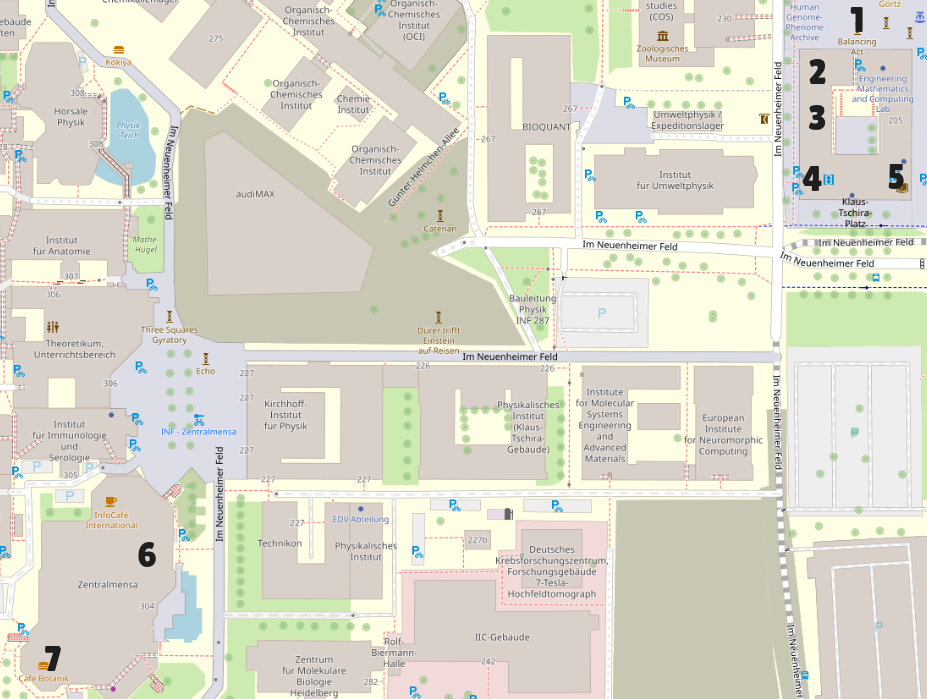
\includegraphics[width=0.7\linewidth]{Karte_NeuenheimerFeld}
		\end{column}
		\begin{column}{.3\textwidth}
			1 - Konsumikon \\
			2 - Hörsaal \\
			3 - SR A - C \\
			4 - Ruheraum \\
			5 - 1. OG Fachschaftsraum \\
			6 - Mensa \\
			7 - Café Botanik \\
		\end{column}
	\end{columns}
\end{frame}

\begin{frame}{Wlan}
	\begin{columns}
		\begin{column}{.7\textwidth}
			\begin{block}{Eduroam}
				\begin{minipage}{.5\linewidth}
					\vspace*{0.5cm}
					\begin{itemize}
						\item Für euch im Alltag
						\item Uni Heidelberg auswählen
						\item Tool runterladen + ausführen
						\item Username: \\ uni-id@uni-heidelberg.de
						\item Passwort: Uni Passwort
					\end{itemize}
					\vspace*{0.5cm}
				\end{minipage}
				\begin{minipage}{.4\linewidth}
					\centering
\includegraphics[width=\linewidth]{eduroam}
					\vfill
				\end{minipage}				
			\end{block}
		\end{column}
		\begin{column}{.3\textwidth}
			\begin{block}{Uni-Webaccess}
				Login mit Unizugang
			\end{block}
			\begin{block}{Heidelberg4You}
				Freies Wlan für alle
			\end{block}
		\end{column}
	\end{columns}
\end{frame}

\section{Programmiervorkurs}

\begin{frame}{Disclaimer}
	\begin{block}{Was erwartet euch?}
		\begin{itemize}
			\item Selbstständiges Arbeiten im eigenen Tempo
			\item Wir helfen bei Schwierigkeiten und Problemen
			\item Wir geben euch \textbf{keine} Lösungen
			\item Am Ende kennt ihr die fundamentalen Konzepte der Programmierung und könnt sie anwenden
			\item \textbf{Ihr werdet nicht bewertet}			
		\end{itemize}
	\end{block}
\end{frame}

\begin{frame}{Tutorien}
	\begin{columns}
		\begin{column}{.3\textwidth}
			\begin{block}{SR A}
				Tutor:innen:
				\begin{itemize}
					\item Fay (sie/ihr)
					\item Sarah (sie/ihr)
				\end{itemize}
				\textbf{Nur für Leute ohne eigenes Gerät}
			\end{block}
		\end{column}
		\begin{column}{.3\textwidth}
			\begin{block}{SR B}
				Tutor:innen:
				\begin{itemize}
					\item Nathanael (er/ihm)
					\item Nick (beliebig)
					\item Tenshi (they/them)
				\end{itemize}
			\end{block}
		\end{column}
		\begin{column}{.3\textwidth}
			\begin{block}{SR C}
				Tutor:innen:
				\begin{itemize}
					\item Kenneth (er/ihm)
					\item Matthias (er/ihm)
				\end{itemize}
			\end{block}
		\end{column}
	\end{columns}
	~\\
	~\\
	\centering\textbf{Ihr könnt euch ab jetzt für die Tutorien eintragen}
\end{frame}

\begin{frame}{Ohne eigenes Gerät}
	Auf eurem Rechner findet ihr eine Datei \emph{vorkurs.pdf} \\
	Die Computer haben \textbf{kein Internet}, recherchiert aber gerne mit eurem Smartphone \\
\end{frame}

\begin{frame}{Mit eigenem Gerät}
	Ladet euch die aktuellste vorkurs.pdf Datei vom Github-Repo selbstständig runter \\
	Link bekommt ihr gleich im Tutorium \\
\end{frame}


\section{Fragen}
\begin{frame}{Fragen}
    \vfill
    \begin{center}
        \Huge Fragen?
    \end{center}
    \vfill
\end{frame}

\end{document}
